\chapter{Optimization of Stirling engine array}

\section{Connection types of SEA}
\label{sec:connectionTypes}
For a single Stirling engine, the heat transfer processes between fluids and engine are independent and irrelevant with the direction of the flows, which means the efficiency and power are not affected by the direction of fluids. However, for an SEA, the connection type will affect the temperature profiles through the array and the specific work production, both of which will determine the efficiency and power of the SEA. It is practically significant to investigate the influence of connection type of an SEA on its performance. Using parallel flow, on the one hand, will reduce the flow rate of the fluid, which will reduce the power of each engine; however, on the other hand, will take the advantage of higher inlet heating fluid temperature (or lower inlet cooling fluid temperature), which may increase the power of each engine. friend who is Using serial flow, on the one hand, will increase the flow rate of the fluid, which will increase the power of each engine; however, on the other hand, the inlet heating fluid temperature reduces with the flow direction (or the inlet cooling fluid temperature increases with the flow direction), which leads to lower engine power along the flow direction. Using the same order will lead to largest fluid temperature difference (temperature difference of the heating and cooling fluids) at the first engines and smallest fluid temperature difference at the last engines. Using the reverse order will lead to more averaged fluid temperature differences of the engines. For a heat exchanger, the reverse order (counterflow), which leads to a smaller fluid temperature difference, has a better heat transfer effect for its lower exergy loss. However, for a Stirling engine, the smaller fluid temperature difference leads to lower performance due to the lower temperature difference of the working gas in the hot space and cold space. To find out the influence of connection types on the performance of SEA, it is essential to classify the connection types.

Five basic connection types of SEA were summarized according to the direction-irrelevant feature of Stirling engine, as shown in Figure~\ref{fig:SEA}. Type 1 is parallel flow, Type 2 is serial flows in the same order, Type 3 is serial flows in the reverse order, Type 4 is heating fluid in serial flow and cooling fluid in parallel flow and Type 5 is heating fluid in parallel flow and cooling fluid in serial flow. All other connection types are the combination of these five basic connection types. For instance, an SEA in Figure~\ref{fig:SEA_eg} is the combination of Type 2 and Type 4. 
%Besides, in the tradition form of solar dish system, Stirling engines are put on the focus points of the dish collectors, which can be considered as a particular case of Type 1.

\noindent \begin{figure}[htbp]
\begin{center}
	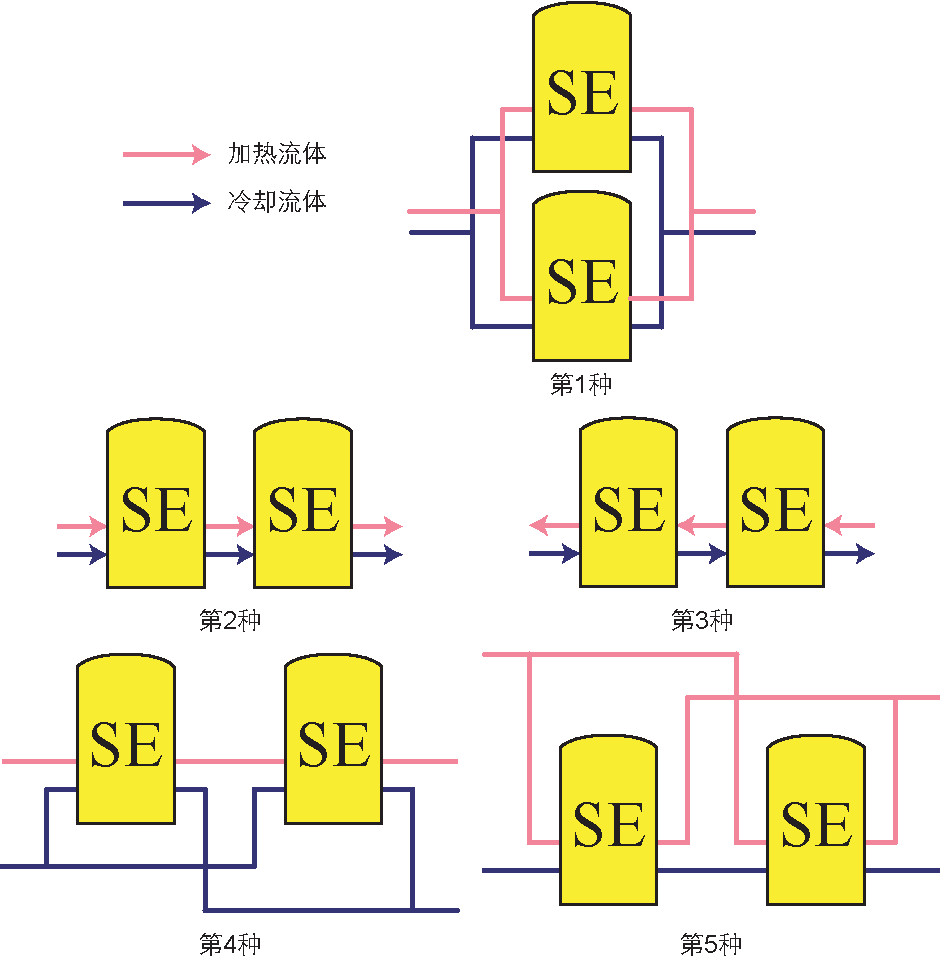
\includegraphics[width = 0.7\columnwidth]{fig/BasicSEA}
	\caption{Five basic connection types of SEA}
	\label{fig:SEA}
\end{center}
\end{figure}

\noindent \begin{figure}[htbp]
\begin{center}
	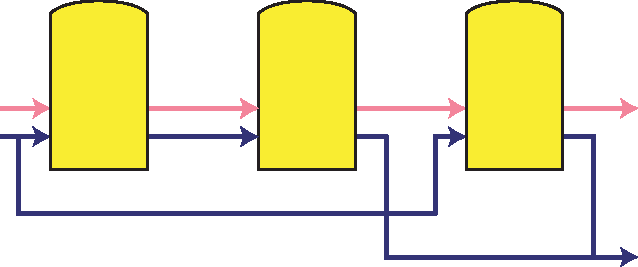
\includegraphics[width = 0.7\columnwidth]{fig/SEA_eg}
	\caption{An instance of connection type of an SEA}
	\label{fig:SEA_eg}
\end{center}
\end{figure}

%\section{Thermodynamic analysis of Stirling engine}
%\subsection{Stirling engine model}\label{sec:StirlingEngineModel}
%\subsubsection{Theoretical Stirling cycle}
%In a Stirling cycle, there are two isothermal processes that exchange heat with heating and cooling fluids, two isochoric processes that exchange heat with regenerator. Figure~\ref{fig:StirlingCycle} shows the schematic of a Stirling cycle, process 1-2 and process 3-4 are the two isothermal processes, process 2-3 and process 4-1 are the two isochoric processes. The heat absorbed by regenerator in process 4-1 is reused in process 2-3, but only able to heat the working gas from 2 to 3' due to the imperfect regeneration. $e$ is defined as the regenerator effectiveness for the imperfect regeneration~\cite{Formosa2010}, $e=\frac{T_R-T_L}{T_H-T_L}$, where $T_H$ is the temperature in the hot space, $T_L$ is the temperature in the cold space, $T_R$ is the effective working fluid temperature in the regenerator.
%\nomenclature{$e$}{regenerator effectiveness}
%\nomenclature{$T_R$}{effective working fluid temperature in regenerator (K)}
%\nomenclature{$T_L$}{Working fluid temperature in the cold space, K}
%\nomenclature{$T_H$}{Working fluid temperature in the hot space, K}
%
%\noindent \begin{figure}[htbp]
%\begin{center}
%	\includegraphics[width = 0.7\columnwidth]{fig/StirlingCycle}
%	\caption{$T$-$s$ diagram of a Stirling cycle}
%	\label{fig:StirlingCycle}
%\end{center}
%\end{figure}
%
%In order to obtain a simplified analytical model, several simplifications were made:
%
%\begin{itemize}
%\item The working gas in Stirling engines obeys the idea gas law. 
%\item No heat loss to the environment for Stirling engines.
%\item Overall heat transfer coefficients of the fluids are constant.
%\item A symmetrical regenerator behavior is assumed~\cite{Formosa2010} so that a simple effectiveness can be obtain by $T_{R}=\frac{T_{H}-T_{L}}{\ln(T_{H}/T_{L})}$.
%\end{itemize}
%
%To consider internal irreversibilities in Stirling cycle made by dead volumes, as described in~\cite{Duan2014}, total dead volume $V_D$ is divided into heater dead volume $V_{DH}$, regenerator dead volume $V_{DR}$ and cooler dead volume $V_{DC}$. There exists a factor $K$ to describe the dead volumes under different temperatures. $K$ is relevant with temperatures in the process and regenerator effectiveness.
%\nomenclature{$V_D$}{total dead volume (m$^3$)}
%\nomenclature{$V_{DH}$}{hot space dead volume (m$^3$)}
%\nomenclature{$V_{DR}$}{regenerator dead volume (m$^3$)}
%\nomenclature{$V_{DC}$}{cold space dead volume (m$^3$)}
%
%\begin{equation}
%	K = \frac{V_{DH}}{T_H} + \frac{V_{DR}}{T_R} + \frac{V_{DC}}{T_L}
%\end{equation}
%\nomenclature{$K$}{Dead volume factor}
%
%For the isothermal compression process 1-2, the output work
%
%\begin{equation}
%	W_{12} = \int^{V_E}_{V_E+V_C}{p_{12}dV}=-mRT_L\ln{\frac{V_E+V_C+KT_L}{V_E+KT_L}}
%\end{equation}
%%\nomenclature{$W_{12}$}{output work in process 1-2 (J)}
%\nomenclature{$V_E$}{expansion volume (m$^3$)}
%\nomenclature{$V_C$}{compression volume (m$^3$)}
%\nomenclature{$m$}{Mass of working fluid in Stirling engine, kg}
%\nomenclature{$R$}{gas constant (J$\cdot$kg$^{-1}\cdot$K$^{-1}$)}
%
%For the isothermal expansion process 3-4, the output work
%
%\begin{equation}
%	W_{34} = \int^{V_E+V_C}_{V_E}{p_{34}dV}=mRT_H\ln{\frac{V_E+V_C+KT_H}{V_E+KT_H}}
%\end{equation}
%%\nomenclature{$W_{34}$}{output work in process 3-4 (J)}
%
%Define $\gamma_H = \frac{V_E+V_C+KT_H}{V_E+KT_H}$, and $\gamma_L = \frac{V_E+V_C+KT_L}{V_E+KT_L}$, so in a cycle, the theoretical output work
%\nomenclature[G]{$\gamma_H$}{Space ratio in process 12}
%\nomenclature[G]{$\gamma_L$}{Space ratio in process 34}
%
%\begin{equation}
%	W_{th} = W_{12} + W_{34} = mR(T_H\ln\gamma_H - T_L\ln\gamma_L)
%\end{equation}
%\nomenclature{$W$}{output work (J)}
%\nomenclature[S]{$th$}{theoretical}
%
%For the isochoric heating process 3'-3, the absorbed heat
%
%\begin{equation}
%	\begin{split}
%		Q_{3^{'}3} = nc_v(T_H-T_R)
%%		\\=n(1-e)c_v(T_H-T_L)
%		=\frac{1-e}{k-1}mR(T_H-T_L)
%	\end{split}
%\end{equation}
%
%%\nomenclature{$Q_{3^{'}3}$}{heat absorbed in process $3^{'}3$ (J)}
%%\nomenclature{$M$}{Mole mass of the working fluid in Stirling engine (kg/mol)}
%\nomenclature{$c_v$}{specific heat at constant volume, J$\cdot$kg$^{-1}\cdot$K$^{-1}$}
%\nomenclature{$k$}{specific heat ratio ($c_p/c_v$), thermal conductivity ,$\mathrm{W\cdot m^{-1}\cdot K^{-1}}$}
%
%For the isothermal expansion process 3-4, the absorbed heat
%
%\begin{equation}
%	Q_{34} = W_{34} = mRT_H\ln\gamma_H
%\end{equation}
%%\nomenclature{$Q_{34}$}{heat absorbed in process 3-4 (J)}
%
%In a cycle, the theoretical absorbed heat
%
%\begin{equation}
%	Q_{th} = Q_{3^{'}3} + Q_{34} = \frac{1-e}{k-1}mR(T_H-T_L) + mRT_H\ln\gamma_H
%\end{equation}
%\nomenclature{$Q$}{absorbed heat (J)}
%
%%The Stirling cycle efficiency
%
%%\begin{equation}
%%	\eta = \frac{W}{Q} = \frac{T_H\ln\gamma_H - T_L\ln\gamma_L}{T_H\ln\gamma_H + \frac{1-e}{k-1}(T_H-T_L)}
%%	\label{Eq:eta}
%%\end{equation}
%%\nomenclature[G]{$\eta$}{efficiency of a Stirling engine}
%%
%%and the output power
%%
%%\begin{equation}
%%	P = {W}s_{se} = mRs_{se}(T_H\ln\gamma_H - T_L\ln\gamma_L)
%%	\label{Eq:P}
%%\end{equation}
%\nomenclature{$P$}{Power of Stirling engine (W)}
%\nomenclature{$s_{se}$}{speed of Stirling engine (Hz)}
%
%%In order to describe quantitatively the effect of the internal dissipation of the working fluid on the performance (efficiency and power) of Stirling engine, the cycle irreversibility parameter, $R_S$, is defined as~\cite{Kaushik2003}:
%%\nomenclature{$R_S$}{cycle irreversibility parameter}
%%
%%\begin{equation}
%%	R_S = \frac{\ln\gamma_H}{\ln\gamma_L} = \frac{s_4 - s_3}{s_1 - s_2}
%%\end{equation}
%%\nomenclature{$s$}{specific entropy (J$\cdot$kg$^{-1}\cdot$K$^{-1}$)}
%%
%%If the internal processes are reversible, $R_S = 1$, Equation~\ref{Eq:eta} becomes the same as described in~\cite{Stine1994}:
%%
%%\begin{equation}
%%	\eta = \frac{T_H - T_L}{T_H + \frac{1-e}{k-1}\cdot\frac{T_H-T_L}{\ln\gamma}}
%%\end{equation}
%%\nomenclature[G]{$\gamma$}{compression ratio}
%
%%It can be found from Equation~\ref{Eq:eta} and~\ref{Eq:P} that 
%%given the properties of a Stirling engine, its efficiency and power can be obtained by known $T_H$ and $T_L$.
%
%\subsubsection{Irreversibilities and losses}
%
%\begin{enumerate}
%\item Non-ideal heat transfer effect
%
%Because of non-ideal heater and cooler, the working fluid temperature ($T_{H}$, $T_L$) in these two heat exchangers is less/higher than the wall temperature ($T_{hw}$, $T_{cw}$), respectively. And $T_{H}$ and $T_{L}$ can be corrected by the wall temperatures as follows:
%
%\begin{equation}
%	T_H = T_{hw} - \frac{Qs_{se}}{h_hA_{hw}}
%	\label{eq:T_H}
%\end{equation}
%\nomenclature[S]{$hw$}{Heater wall}
%
%\begin{equation}
%	T_L = T_{cw} + \frac{(Q-W)s_{se}}{h_cA_{cw}}
%	\label{eq:T_L}
%\end{equation}
%\nomenclature[S]{$cw$}{Cooler wall}
%
%The heat transfer coefficient can be obtained using the following correlation~\cite{Babaelahi2015}:
%
%\begin{equation}
%	h_{h,c} = \frac{\mu c_pf_{Re}}{2D_{h,c}Pr_{h,c}}
%\end{equation}
%\nomenclature[G]{$\mu$}{dynamic viscosity ($\mathrm{kg\cdot m^{-1}\cdot s^{-1}}$)}
%
%where $f_{Re}$ is a Reynolds friction factor defined as:
%
%\begin{equation}
%	f_{Re} = 0.0791{Re_{h,c}}^{0.75}
%\end{equation}
%
%$Re_{h,c}$, $Pr_{h,c}$ and $D_{h,c}$ are Reynolds number, Prandtl number and hydraulic diameter of the heater/cooler exchanger.
%
%\item Effect of pressure drop
%
%Pressure drops in the heat exchangers cause power losses of the Stirling engine. The pressure drops can be obtained by~\cite{Urieli1984}:
%
%\begin{equation}
%	\Delta p = -\frac{2f_{Re}\mu u V}{d^2A}
%\end{equation}
%\nomenclature{$p$}{pressure (Pa)}
%
%where $u$ is the working gas speed, $V$ is volume, $A$ is flow cross-section area.
%
%The net power loss of the Stirling engine due to pressure drop of the heat exchangers can be evaluated by:
%
%\begin{equation}
%	W_{pd} = \oint\underset{i = E,C}{\sum}(\Delta p_{i}\frac{dV_i}{d\theta})d\theta
%\end{equation}
%
%\item Effect of finite speed of piston and mechanical friction
%
%Due to the finite speed of piston, the pressure on the piston surface is different from the pressure of expansion and compression spaces. It has been demonstrated that the pressure on the piston surface in the expansion process is less than the mean pressure in the expansion space. Similarly, the pressure on the piston surface in the compression process is greater than the mean pressure in the compression space. This means the output work is less than the theoretical value. Besides, The output work also reduces due to mechanical friction. The output work loss due to finite speed of piston and mechanical friction can be obtained as follows~\cite{Babaelahi2015}:
%
%\begin{equation}
%	W_{fs} = \oint p(\pm\frac{au_p}{c}\pm\frac{\Delta p_f}{p})dV
%\end{equation}
%
%where the sign (+) is used in the compression space, and the sign (-) is used in the expansion space. $p$ is the mean pressure in the compression/expansion space, $u_p$ is velocity of the piston, $c$ is the average speed of molecules and $\Delta p_f$ is the pressure loss due to mechanical friction. $\Delta p_f$, $a$ and $c$ can be obtained by~\cite{Heywood1988}:
%
%\begin{equation}
%	\Delta p_f = 0.97+0.009s_{se}
%\end{equation}
%\begin{equation}
%	a = \sqrt{3k}
%\end{equation}
%\begin{equation}
%	c = \sqrt{3RT}
%\end{equation}
%
%\item Energy losses due to internal conduction
%
%The temperature differs from the heater and cooler, heat losses from heater to cooler exists due to internal conduction through the walls of regenerator.~\cite{Strauss2010} The internal conduction loss in a cycle can be obtained by follows:
%
%\begin{equation}
%	Q_{id} = \frac{k_rA_r}{L_rs_{se}}(T_{hw} - T_{cw})
%\end{equation}
%
%where, $k_r$, $A_r$ and $L_r$ denote the regenerator matrix conductivity, regenerator length, and regenerator conductive area respectively.
%\nomenclature[S]{$r$}{regenerator}
%
%\item Energy losses due to shuttle conduction
%
%The displacer shuttles between the expansion and compression space. It absorbs heat during the hot end of its stroke and releases it during the cold end of its stroke. This heat loss can be estimated as~\cite{Timoumi2008}:
%
%\begin{equation}
%	Q_{sc} = 0.4\frac{Z^2k_pD_p}{JL_ds_{se}}(T_{H} - T_{L})
%\end{equation}
%
%where, $Z$, $k_p$, $D_p$, $J$ and $L_d$ denote the displacer stroke, piston thermal conductivity, displacer diameter, gap between the displacer and the cylinder, and length of the displacer respectively.
%\nomenclature{$Z$}{Displacer stroke (m)}
%\nomenclature{$J$}{Annular gap cylinder displacer (m)}
%\nomenclature[S]{$p$}{Piston}
%
%\end{enumerate}
%
%So, in a Stirling engine, the total absorbed heat in a cycle
%
%\begin{equation}
%	Q = Q_{th} + Q_{id} + Q_{sc}
%\end{equation}
%
%the output work
%
%\begin{equation}
%	W = W_{th} - W_{pd} - W_{fs}
%\end{equation}
%
%Power of the Stirling engine
%
%\begin{equation}
%	P = Ws_{se}
%	\label{Eq:P}
%\end{equation}
%
%Efficiency of the Stirling engine
%
%\begin{equation}
%	\eta = W/Q
%	\label{Eq:eta}
%\end{equation}
%
%
%\subsection{Model validation}~\label{sec:modelValidation}
%
%Evaluation of the developed thermal model was performed by considering the GPU-3 Stirling engine as a case study. Design specifications of the GPU-3 Stirling engine are indicated in Table~\ref{tab:GPU3parameters}. The thermal efficiency and power of the proposed Stirling engine model was compared with previous thermal models and experimental data as shown in Table~\ref{tab:EfficiencyComparison} and Table~\ref{tab:PowerComparison}.
%
%\begin{table*}[htbp]\footnotesize
%	\caption{Design specifications of the GPU-3 Stirling engine~\cite{Babaelahi2015,Martini1983}}
%	\begin{center}
%	\begin{tabular}{ll}
%		\toprule
%		Parameter				&	Value\\
%		\midrule
%		Engine type					&	$\beta$\\
%		Working gas			&	Helium\\
%		Mass of the working gas	&	1.136\,g\\
%		\emph{Heater}			&\\
%		Number of tubes		&	40\\
%		Tube external diameter	&	4.83$\times10^{-3}\,\mathrm{m}$\\
%		Tube internal diameter	&	3.02$\times10^{-3}\,\mathrm{m}$\\
%		Tube length (cylinder side)&	0.1164\,m\\
%		Tube length (regenerator side)		&	0.1289\,m\\
%		\emph{Cooler}			&\\
%		Number of tubes		&	312\\
%		Tube external diameter	&	1.59$\times10^{-3}\,\mathrm{m}$\\
%		Tube internal diameter	&	1.09$\times10^{-3}\,\mathrm{m}$\\
%		Average tube length		&	4.61$\times10^{-2}\,\mathrm{m}$\\
%		\emph{Regenerator}		&\\
%		Number of regenerator	&	8\\
%		Regenerator internal diameter	&	2.26$\times10^{-2}\,\mathrm{m}$\\
%		Regenerator length		&	2.26$\times10^{-2}\,\mathrm{m}$\\
%		Diameter of regenerator tube	&	4$\times10^{-5}\,\mathrm{m}$\\
%		Material				&	Stainless steel\\
%		\emph{Volume}			&\\
%		Swept Vol. (expansion/compression)	&	120.82/114.13\,$\mathrm{cm}^3$\\
%		Clearance Vol. (expansion/compression)	&	30.52/28.68\,$\mathrm{cm}^3$\\
%		Dead Vol. (heater/cooler/regenerator)	&	70.28/13.18/50.55\,$\mathrm{cm}^3$\\
%		\bottomrule
%	\end{tabular}
%	\end{center}
%	\label{tab:GPU3parameters}
%\end{table*}
%
%
%\begin{table*}[htbp]\footnotesize
%	\caption{Thermal efficiency of the proposed model, previous thermal models and experimental data(at $T_{hw}=922\,\mathrm{K}$ and $T_{cw}=288\,\mathrm{K}$)}
%	\begin{center}
%	\begin{tabular}{cccccccccccc}
%		\toprule
%		\multirow{7}{0.5in}{\tabincell{l}{Rotation\\speed\\(Hz)}}	&	\multirow{7}{0.5in}{Mean effective pressure (MPa)}	&	\multicolumn{3}{c}{\multirow{1}{1.0in}{Thermal efficiency predicted by the simple analysis (variable Pr~\cite{Urieli1984})}}	&	\multicolumn{3}{c}{\multirow{1}{1.0in}{Thermal efficiency predicted by the adiabatic analysis (simple II~\cite{Strauss2010})}}	&	\multicolumn{3}{c}{\multirow{1}{1.0in}{Thermal efficiency predicted by the proposed Stirling Engine model}}	&	\multirow{4}{*}{\tabincell{l}{Experimental\\efficiency~\cite{Babaelahi2015}}}\\
%		\\
%		\\
%		\\
%		\cline{3-12}
%		&&\multirow{3}{*}{\tabincell{c}{Value\\(\%)}}&	\multirow{3}{*}{\tabincell{c}{Error\\(\%)}}&\multirow{3}{*}{\tabincell{c}{Average\\error\\(\%)}}&\multirow{3}{*}{\tabincell{c}{Value\\(\%)}}&	\multirow{3}{*}{\tabincell{c}{Error\\(\%)}}&\multirow{3}{*}{\tabincell{c}{Average\\error\\(\%)}}&\multirow{3}{*}{\tabincell{c}{Value\\(\%)}}&	\multirow{3}{*}{\tabincell{c}{Error\\(\%)}}&\multirow{3}{*}{\tabincell{c}{Average\\error\\(\%)}}&\multirow{3}{*}{\tabincell{c}{Actual\\value\\(\%)}}\\
%		\\
%		\\
%		\midrule
%		16.67	&\multirow{6}{*}{2.76}	&38.72	&18.22	&\multirow{6}{*}{17.90}	&32.48	&11.98	&\multirow{6}{*}{12.85}	&28.16	&7.66	&\multirow{6}{*}{12.10}	&20.50\\
%		25.00	&&36.16	&15.46	&&31.21	&10.51	&&27.75	&7.05	&&20.70\\
%		33.33	&&33.79	&15.79	&&29.45	&11.45	&&27.43	&9.43	&&18.00\\
%		41.67	&&31.48	&16.28	&&27.45	&12.25	&&27.17	&11.97	&&15.20\\
%		50.00	&&29.12	&17.32	&&25.21	&13.41	&&26.94	&15.14	&&11.80\\
%		58.33	&&29.74	&24.34	&&22.89	&17.49	&&26.74	&21.34	&&5.40\\
%		\midrule
%		25.00	&\multirow{5}{*}{4.14}	&35.65	&10.85	&\multirow{5}{*}{11.46}	&32.29	&7.49	&\multirow{5}{*}{8.28}	&27.29	&2.49	&\multirow{5}{*}{6.65}	&24.80\\
%		33.33	&&33.52	&9.62	&&30.40	&6.50	&&26.94	&3.04	&&23.90\\
%		41.67	&&31.48	&10.18	&&28.39	&7.09	&&26.65	&5.35	&&21.30\\
%		50.00	&&29.45	&11.25	&&26.33	&8.13	&&26.39	&8.19	&&18.20\\
%		58.33	&&27.40	&15.40	&&24.21	&12.21	&&26.17	&14.17	&&12.00\\
%		\midrule
%		41.67	&\multirow{3}{*}{5.52}	&31.20	&8.70	&\multirow{3}{*}{10.82}	&28.59	&6.09	&\multirow{3}{*}{8.11}	&26.24	&3.74	&\multirow{3}{*}{7.48}	&22.50\\
%		50.00	&&29.33	&10.53	&&26.62	&7.82	&&25.97	&7.17	&&18.80\\
%		58.33	&&27.44	&13.24	&&24.62	&10.42	&&25.73	&11.53	&&14.20\\
%		\midrule
%		50.00	&\multirow{2}{*}{6.90}	&29.07	&10.37	&\multirow{2}{*}{11.73}	&26.61	&7.91	&\multirow{2}{*}{9.19}	&25.62	&6.92	&\multirow{2}{*}{9.05}		&18.70\\
%		58.33	&&27.29	&13.09	&&24.67	&10.47	&&25.37	&11.17	&&14.20\\
%		\bottomrule
%	\end{tabular}
%	\end{center}
%	\label{tab:EfficiencyComparison}
%\end{table*}
%
%\begin{table*}[htbp]\footnotesize
%	\caption{Output power of the proposed model, previous thermal models and experimental data(at $T_{hw}=922\,\mathrm{K}$ and $T_{cw}=288\,\mathrm{K}$)}
%	\begin{center}
%	\begin{tabular}{cccccccccccc}
%		\toprule
%		\multirow{7}{0.5in}{\tabincell{l}{Rotation\\speed\\(Hz)}}	&	\multirow{7}{0.5in}{Mean effective pressure (MPa)}	&	\multicolumn{3}{c}{\multirow{1}{1.0in}{Output power predicted by the simple analysis (variable Pr~\cite{Urieli1984})}}	&	\multicolumn{3}{c}{\multirow{1}{1.0in}{Output power predicted by the adiabatic analysis (simple II~\cite{Strauss2010})}}	&	\multicolumn{3}{c}{\multirow{1}{1.0in}{Output power predicted by the proposed Stirling Engine model}}	&	\multirow{4}{*}{\tabincell{l}{Experimental\\output\\power\\(kW)~\cite{Babaelahi2015}}}\\
%		\\
%		\\
%		\\
%		\cline{3-12}
%		&&\multirow{3}{*}{\tabincell{c}{Value\\(kW)}}&	\multirow{3}{*}{\tabincell{c}{Error\\(\%)}}&\multirow{3}{*}{\tabincell{c}{Average\\error\\(\%)}}&\multirow{3}{*}{\tabincell{c}{Value\\(kW)}}&	\multirow{3}{*}{\tabincell{c}{Error\\(\%)}}&\multirow{3}{*}{\tabincell{c}{Average\\error\\(\%)}}&\multirow{3}{*}{\tabincell{c}{Value\\(kW)}}&	\multirow{3}{*}{\tabincell{c}{Error\\(\%)}}&\multirow{3}{*}{\tabincell{c}{Average\\error\\(\%)}}&\multirow{3}{*}{\tabincell{c}{Actual\\value\\(kW)}}\\
%		\\
%		\\
%		\midrule
%		16.67	&\multirow{6}{*}{2.76}	&1.796	&119.02	&\multirow{6}{*}{272.03}	&1.772	&116.10	&\multirow{6}{*}{254.71}	&0.861	&4.98	&\multirow{6}{*}{104.84}	&0.82\\
%		25.00	&&2.555	&128.13	&&2.500	&123.21	&&1.253	&11.88	&&1.12\\
%		33.33	&&3.215	&165.70	&&3.117	&157.60	&&1.632	&34.88	&&1.21\\
%		41.67	&&3.769	&211.49	&&3.615	&198.76	&&2.001	&65.37	&&1.21\\
%		50.00	&&4.195	&303.37	&&3.973	&282.08	&&2.362	&127.12	&&1.04\\
%		58.33	&&4.505	&704.46	&&4.203	&650.54	&&2.715	&384.82	&&0.56\\
%		\midrule
%		25.00	&\multirow{5}{*}{4.14}	&3.844	&114.75	&\multirow{5}{*}{259.70}	&3.761	&110.11	&\multirow{5}{*}{158.41}	&1.818	&1.56	&\multirow{5}{*}{39.83}	&1.79\\
%		33.33	&&4.856	&120.73	&&4.708	&114.00	&&2.362	&7.36	&&2.20\\
%		41.67	&&5.734	&136.94	&&5.501	&127.31	&&2.890	&19.42	&&2.42\\
%		50.00	&&6.462	&174.98	&&6.126	&160.68	&&3.405	&44.89	&&2.35\\
%		58.33	&&7.030	&306.36	&&6.573	&279.94	&&3.908	&125.90	&&1.73\\
%		\midrule
%		41.67	&\multirow{3}{*}{5.52}	&7.645	&133.08	&\multirow{3}{*}{180.02}	&7.334	&123.60	&\multirow{3}{*}{164.91}	&3.742	&14.09	&\multirow{3}{*}{43.68}	&3.28\\
%		50.00	&&8.655	&163.87	&&8.206	&150.18	&&4.401	&34.18	&&3.28\\
%		58.33	&&9.470	&243.12	&&8.858	&220.94	&&5.045	&82.79	&&2.76\\
%		\midrule
%		50.00	&\multirow{2}{*}{6.90}	&10.788	&174.50	&\multirow{2}{*}{287.04}	&10.223	&160.13	&\multirow{2}{*}{263.63}	&5.362	&36.44	&\multirow{2}{*}{97.75}		&3.93\\
%		58.33	&&11.840	&399.58	&&11.071	&367.13	&&6.140	&159.07	&&2.37\\
%		\bottomrule
%	\end{tabular}
%	\end{center}
%	\label{tab:PowerComparison}
%\end{table*}
%
%It can be found that the proposed model has much better agreement with the experimental results than previous thermal models at various rotation speeds and mean effective pressures. It is required to mention that in all thermal models both power $W$ and input heat $Q$ were determined by the thermal process of heat transfer between the wall and working gas. In the proposed model, $W$ and $Q$ are obtained by Equation~\ref{eq:T_H} and~\ref{eq:T_L}. Therefore, all the three parameters $W$, $Q$ and $\eta$ are determined by the thermal model and input parameters to the model. These input parameters include heater, cooler, mean effective pressure, type of working gas and geometrical specification of the engine.
%
%Table~\ref{tab:EfficiencyComparison} and~\ref{tab:PowerComparison} indicate that when mean effective pressure of the engine increases from $2.76\,\mathrm{MPa}$ to $6.90\,\mathrm{MPa}$, best performance (efficiency and power) prediction of the proposed model exists. When rotation speed increases from $16.67\,\mathrm{Hz}$ to $58.33\,\mathrm{Hz}$, error in prediction of performance of the proposed model increases. The proposed model may have the best performance prediction at a low rotation speed, with mean effective pressure between $4.14\,\mathrm{MPa}$ and $5.52\,\mathrm{MPa}$.
%
%However, there is still some discrepancy between the simulation results of proposed model and the experimental data. In the future researches, more accurate models of Stirling engine may be developed by considering other irreversibilities such as heat loss to the environment, gas spring hysteresis, and etc. It is worth pointing that there are more accurate Stirling engine models. For example, polytropic simulation models of Stirling engine show higher accuracy than our proposed model~\cite{Hosseinzade2015, Babaelahi2015}. However, the model needs more costly calculations and the polytropic indexes are engine-specific.
%
%\subsection{Heat transfer between the engine and the fluids}
%
%For a Stirling engine thermal process, the wall temperatures of the heater and cooler are considered to be uniform and constant. The heat transferred between the wall and the fluids is
%%with heating and cooling fluids, the heat exchange processes are considered to be isothermal processes.
%%%For an isothermal process in Figure~\ref{fig:ConstTempHX}, transferred heat equals to fluid's enthalpy rise: 
%%For an isothermal process, transferred heat equals to fluid's enthalpy rise: 
%
%\begin{equation}
%	(T_w-T)UdA = \dot{m}mc_pdT
%\end{equation}
%\nomenclature{$\dot{m}$}{Mass flow rate (kg$\cdot$s$^{-1}$)}
%\nomenclature{$c_p$}{specific heat at constant pressure (J$\cdot$kg$^{-1}\cdot$K$^{-1}$)}
%\nomenclature{$T_w$}{wall temperature (K)}
%\nomenclature{$U$}{overall heat transfer coefficient (W$\cdot$m$^{-2}\cdot$K$^{-1}$)}
%\nomenclature{$A$}{heat transfer area (m$^2$)}
%
%with $T(0)=T_i$, $T(A)=T_o$,
%\nomenclature[S]{$i$}{inlet}
%\nomenclature[S]{$o$}{outlet}
%
%\begin{equation}
%	\frac{T_o-T_w}{T_i-T_w}=\exp(-\frac{UA}{\dot{m}c_p})
%\end{equation}
%
%%\noindent \begin{figure}[htbp]
%%\begin{center}
%%	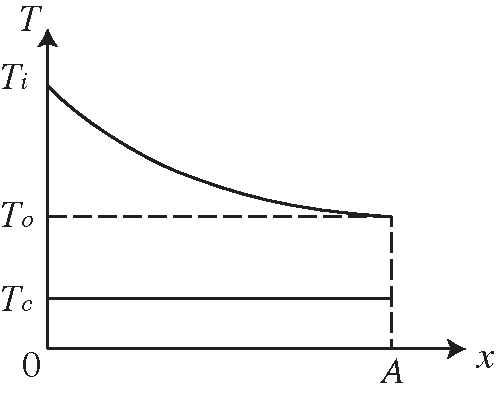
\includegraphics[width = 0.3\columnwidth]{graphics/ConstTempHX}
%%	\caption{Diagram of heat transfer to a constant temperature heat source}
%%	\label{fig:ConstTempHX}
%%\end{center}
%%\end{figure}
%
%%So
%%
%%\begin{equation}
%%	\frac{dT}{dA}=-\frac{U}{\dot{m}c_p}(T-T_c)
%%\end{equation}
%%
%
%For a Stirling engine, $T_{hw}$ or $T_{cw}$ can be used to substitute $T_w$ to get the relationships between $T_{i,h}$, $T_{o,h}$ and $T_{hw}$, or $T_{i,c}$, $T_{o,c}$ and $T_{cw}$ respectively.
%\nomenclature[S]{$h$}{Heating fluid}
%\nomenclature[S]{$c$}{Cooling fluid}
%
%\begin{equation}
%	\frac{T_{o,h}-T_{hw}}{T_{i,h}-T_{hw}}=\exp(-\frac{U_hA_h}{\dot{m}_h}c_{p,h}})
%	\label{Eq:T_h}
%\end{equation}
%
%\begin{equation}
%	\frac{T_{o,c}-T_{cw}}{T_{i,c}-T_{cw}}=\exp(-\frac{U_cA_c}{\dot{m}_cc_{p,c}})
%	\label{Eq:T_c}
%\end{equation}
%
%Heat transferred from heating fluid to Stirling engine in a cycle
%
%\begin{equation}
%	q_{m,h}c_{p,h}(T_{i,h}-T_{o,h})/s_{se} = Q
%	\label{Eq:q_h}
%\end{equation}
%
%Heat transferred from Stirling engine to cooling fluid in a cycle
%
%\begin{equation}
%	q_{m,c}c_{p,c}(T_{o,c}-T_{i,c})/s_{se} = Q - W
%	\label{Eq:q_c}
%\end{equation}

%For a Stirling engine given $q_{m,h}$, $q_{m,c}$ and $s_{se}$, known 2 of the 6 parameters ($T_{i,h}$, $T_{o,h}$, $T_{i,c}$, $T_{o,c}$, $T_H$ and $T_L$), the rest 4 can be obtained by solving 
%%Equation~\ref{Eq:T_h},~\ref{Eq:T_c},~\ref{Eq:q_h} and~\ref{Eq:q_c}
%Equation~\ref{Eq:T_h}-\ref{Eq:q_c}
%. Then $\eta$ and $P$ can be obtained by Equation~\ref{Eq:eta} and~\ref{Eq:P}. This means the performance of a given Stirling engine can be inquired by the input/output parameters of heating/cooling fluids.

\section{Modeling of the SEAs}

As mentioned in Section~\ref{sec:connectionTypes}, there are five basic connection types for an SEA. All other connection types are the combination of these five basic connection types. This thesis investigates the five basic connection types.

To determine the performance of an SEA, models of all the Stirling engines need to be built depending on their thermodynamic characteristic. Stirling engines are chosen to have the same parameters including the same speed $s_{se}$. This is a reasonable assumption when using SEA for power generation, where the output power frequency should be constant. The speed of Stirling engine can be calibrated by speed controller system~\cite{Hooshang2016}. To eliminate interference of other factors, heating and cooling fluids are chosen to have same parameters for different connection types of SEAs. To clearly find out the performance differences of different SEAs, large temperature differences of the heating/cooling fluids after heat exchange with the engines are preferred. Air was chosen as the cooling fluid instead of commonly used water to avoid small temperature rise and evaporation in the cooling process. Design parameters of Stirling engines are the same as shown in Table~\ref{tab:GPU3parameters}. Other parameters of Stirling engines and heating/cooling fluids in SEAs are shown in Table~\ref{tab:parameters}. Rotation speed of the engines and mean effective pressure were chosen to be 25$\,\mathrm{Hz}$ and 5$\,\mathrm{MPa}$ respectively to get the best Stirling engine model for performance prediction, as pointed in Section~\ref{sec:modelValidation}.

\begin{table}[htbp]
	\caption{Parameters of SEA models}
	\begin{center}
	\begin{tabular}{cccc}
		\toprule
		Parameter		&	Value	& Parameter	&	Value\\
		\midrule
		Heating fluid	&	Air		&	$\dot{m}_h$	&	0.4\,kg/s\\
		Cooling fluid	&	Air	&	$T_{i,h}$	&	1000\,K\\
		$n_{se}$	&	6	&	$p_{i,h}$	&	5$\times$10$^5$\,Pa\\
		$s_{se}$	&	25\,Hz	&	$\dot{m}_c$	&	0.4\,kg/s\\
		$p_{se}$		&	5\,MPa	&	$T_{i,c}$	&	300\,K\\
		$U_hA_h$	&	180\,W/K	&	$p_{i,c}$	&	5$\times$10$^5$\,Pa\\
		$U_cA_c$		&	180\,W/K	&&\\
		\bottomrule
	\end{tabular}
	\end{center}
	\label{tab:parameters}
\end{table}

In an SEA, there are 2 flows as shown in Figure~\ref{fig:SEA}. In a serial flow, each engine's mass flow rate is $\dot{m}$, and from the flow's direction, for $2\leqslant{}x\leqslant{}n_{se}$, $T_{i,x} = T_{o,x-1}$. In a parallel flow, each engine's mass flow is $\dot{m}/n_{se}$, for $2\leqslant{}x\leqslant{}n_{se}$, $T_{i,x} = T_{i,h}$.
%\nomenclature{$n_{se}$}{Number of Stirling engine in SEA}

\begin{equation}
	\begin{split}
		T_{i,x} = T_{o,x-1}
		\label{Eq:T_serial}
	\end{split}
\end{equation}

\begin{equation}
	T_{i,x} = T_{i,h}
	\label{Eq:T_parallel}
\end{equation}

According to the equations 
%(Equation~\ref{Eq:T_h},~\ref{Eq:T_c},~\ref{Eq:q_h},~\ref{Eq:q_c},~\ref{Eq:T_serial},~\ref{Eq:T_parallel})
(Equation~(\ref{Eq:T_h})-(\ref{Eq:T_parallel}))
, there are $6n_{se} - 2$ equations for $6n_{se}$ parameters for $n_{se}$ engines. Other parameters of an SEA can be calculated by the given inlet temperature of the heating and cooling fluids. The efficiency and power of each engine can be obtained from Equation~(\ref{Eq:eta}),~(\ref{Eq:P}). The total efficiency and power of SEA can be obtained by powers of engines and outlet properties of the fluids.

MATLAB was used as the programming tool to build the model of SEAs, and CoolProp was used to provide fluid properties for MATLAB program. Five basic SEA models composed of the aforementioned Stirling engines and fluids were built. To compare SEA connection types under various conditions, several parameters are investigated to find out their effects on SEA performance.

\noindent \begin{figure}[htbp]
\begin{center}
	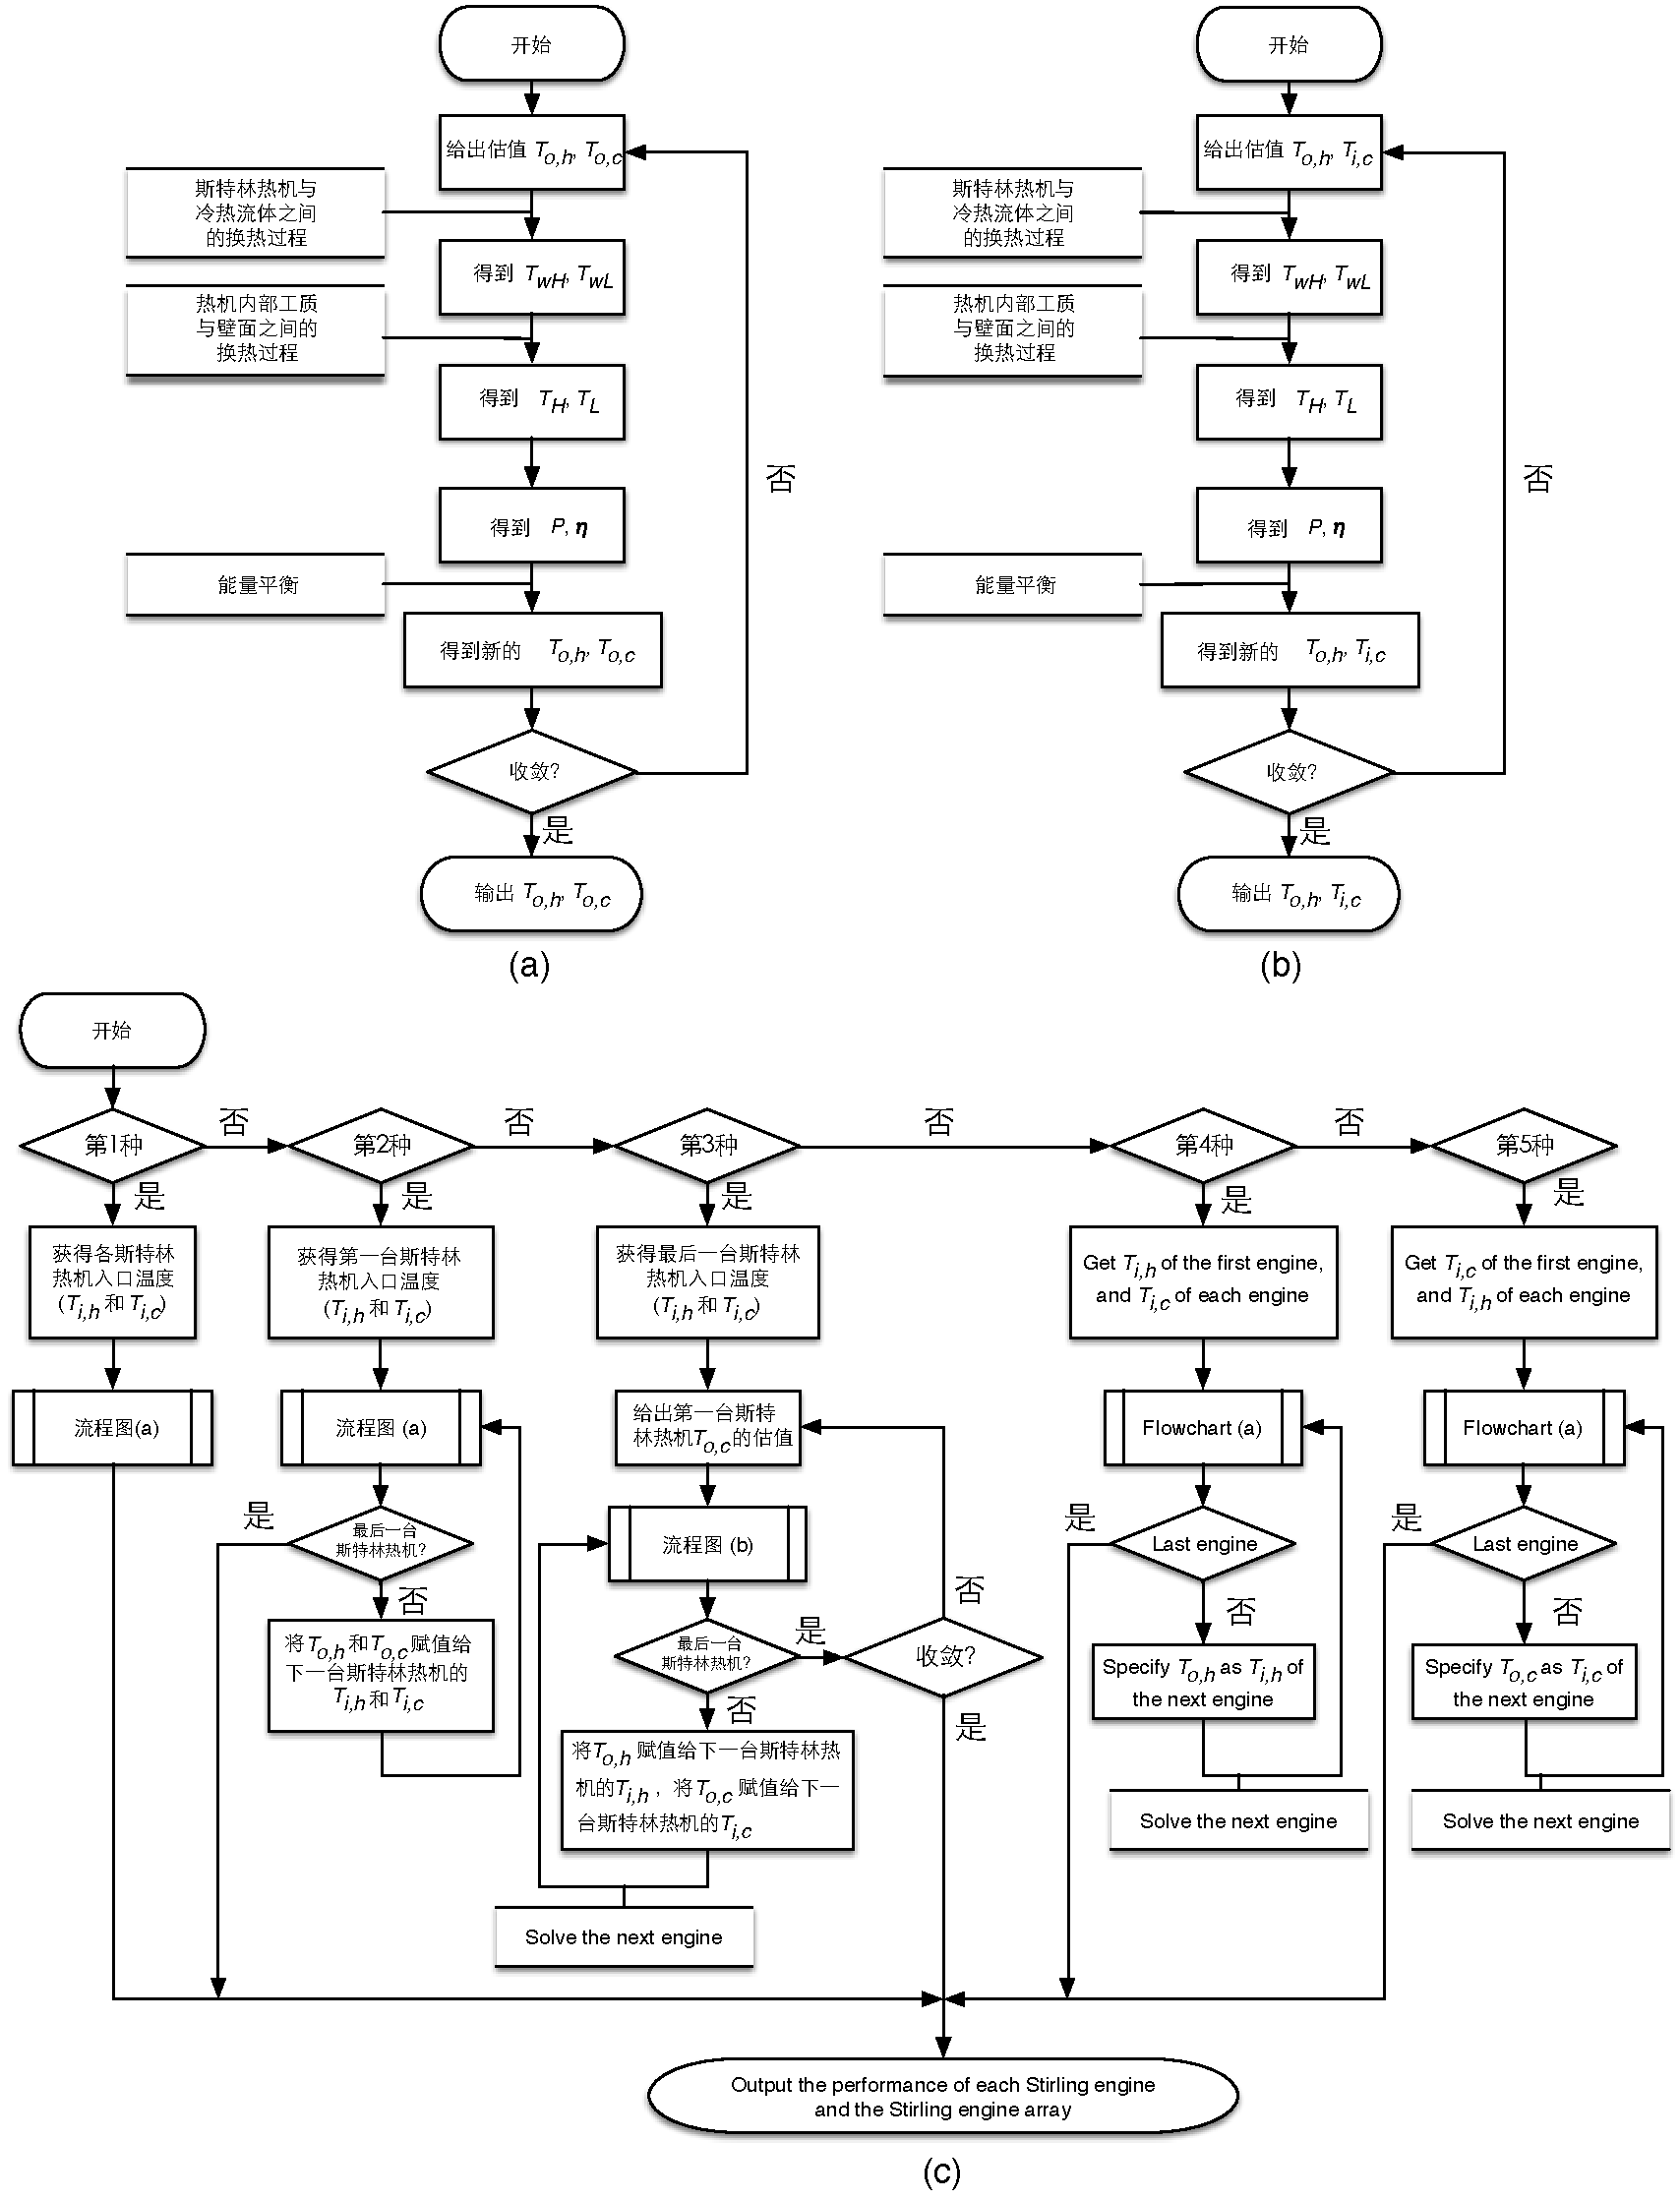
\includegraphics[width = 1.0\columnwidth]{fig/FlowChart}
	\caption{Flowcharts of the SEA model for performance analysis of the SEAs}
	\label{fig:Flowchart}
\end{center}
\end{figure}

Figure~\ref{fig:Flowchart} shows the solution algorithm of the SEA model. Flowchart (a) shows the algorithm to solve a Stirling engine known inlet parameters of the fluids. Flowchart (b) shows the algorithm to solve a Stirling engine known inlet parameters of heating fluid and outlet parameters of cooling fluid. Flowchart (c) shows the algorithm to solve the SEA model iteratively depending on different connection types. The levenberg-marquardt algorithm is applied to numerically solve the non-linear equations in the flowcharts.

\section{Result analysis}
%The objective of this study is to investigate SEA performance difference of different connection types. Therefore, 

SEA models with specified parameters in Table~\ref{tab:parameters} were built and calculated. Results of the performances of the SEAs are shown in Table~\ref{tab:result}, it can be found that under specified parameters Type 3 has the highest efficiency and output power, while Type 1 has the lowest efficiency and output power.

\begin{table}[htbp]
	\caption{Results of SEA models under specified parameters}
	\begin{center}
	\begin{tabular}{cccc}
		\toprule
		Parameter		&	Value	&	Parameter		&	Value\\
		\midrule
		$\eta_1$	&	0.2215	&	$P_1$		&	8022\,W\\
		$\eta_2$	&	0.2273	&	$P_2$		&	8483\,W\\
		$\eta_3$	&	0.2277	&	$P_3$		&	8512\,W\\
		$\eta_4$	&	0.2227	&	$P_4$		&	8116\,W\\
		$\eta_5$	&	0.2263	&	$P_5$		&	8399\,W\\		
		\bottomrule
	\end{tabular}
	\end{center}
	\label{tab:result}
\end{table}

\subsection{Effects of $T_{i,h}$}
According to Carnot cycle efficiency formula, the temperature of heating fluid determines the efficiency of Stirling engine array. For a Stirling engine, lower temperature heating fluid leads to a lower efficiency. The efficiency and output power may drop to 0 due to its insufficient heating fluid temperature to drive the engine.

\noindent \begin{figure}[htbp]
\begin{center}
	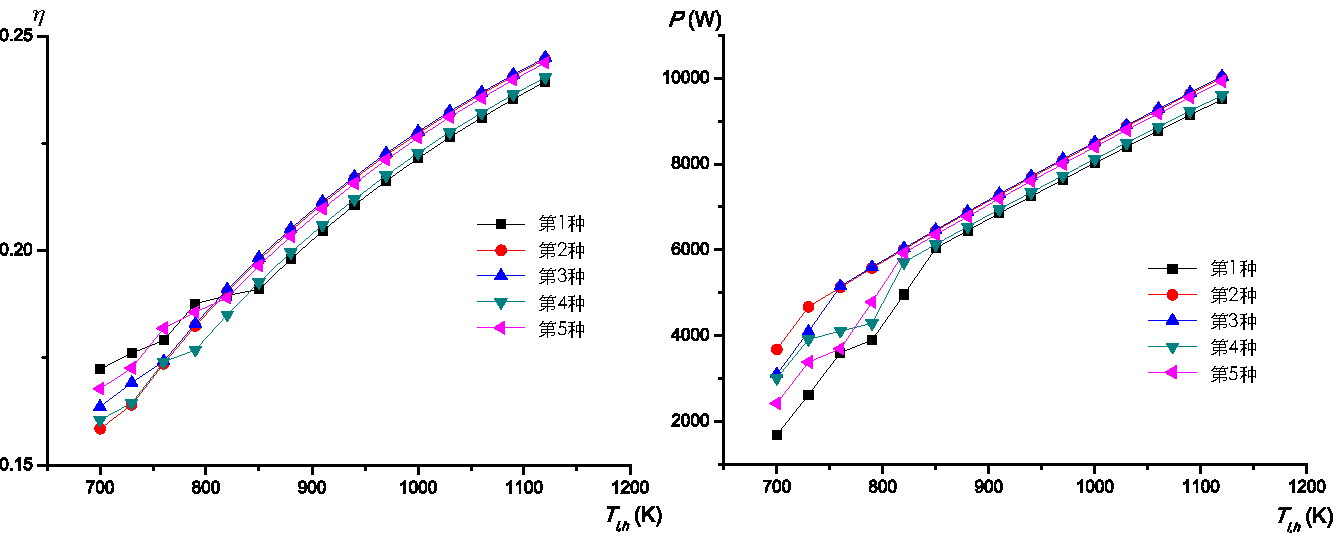
\includegraphics[width = 0.7\columnwidth]{fig/T_ih}
	\caption{Influence of $T_{i,h}$ on efficiency and power of SEA}
	\label{fig:Ti_h}
\end{center}
\end{figure}

Curves of performance of SEAs and $T_{i,h}$ are shown in Figure~\ref{fig:Ti_h}.
As it is shown, with the increase of $T_{i,h}$, both $\eta$ and $P$ increase for all SEAs. For some types of SEA, when $T_{i,h}$ is lower than a critical temperature, some of the engines in the SEA will not work and there will be turning points on the $\eta-T_{i,h}$, $P-T_{i,h}$ curves. For example, in SEA of Type 1, when $T_{i,h}$ is lower 820\,K, all the engines stop working, turning points at 820\,K can be found on the $\eta-T_{i,h}$, $P-T_{i,h}$ curves in Figure~\ref{fig:Ti_h}. 
%Multiple turning points on one curve means different engines in the SEA stop working from different temperatures.

From curves in Figure~\ref{fig:Ti_h}, it can be concluded that Type 2 and Type 3 have the best performance, and Type 2 has the best adaptability for lower $T_{i,h}$. All engines in Type 2 work at 730\,K.

\subsection{Effects of $\dot{m}c_p$}

According to Equation~(\ref{Eq:q_h}),~(\ref{Eq:q_c}), $\dot{m}c_p$ (both $\dot{m}_hc_{p,h}$ and $\dot{m}_cc_{p,c}$) will affect the heat transfer process, which is one of the vital factor for the performance of SEA.


\noindent \begin{figure}[htbp]
\begin{center}
	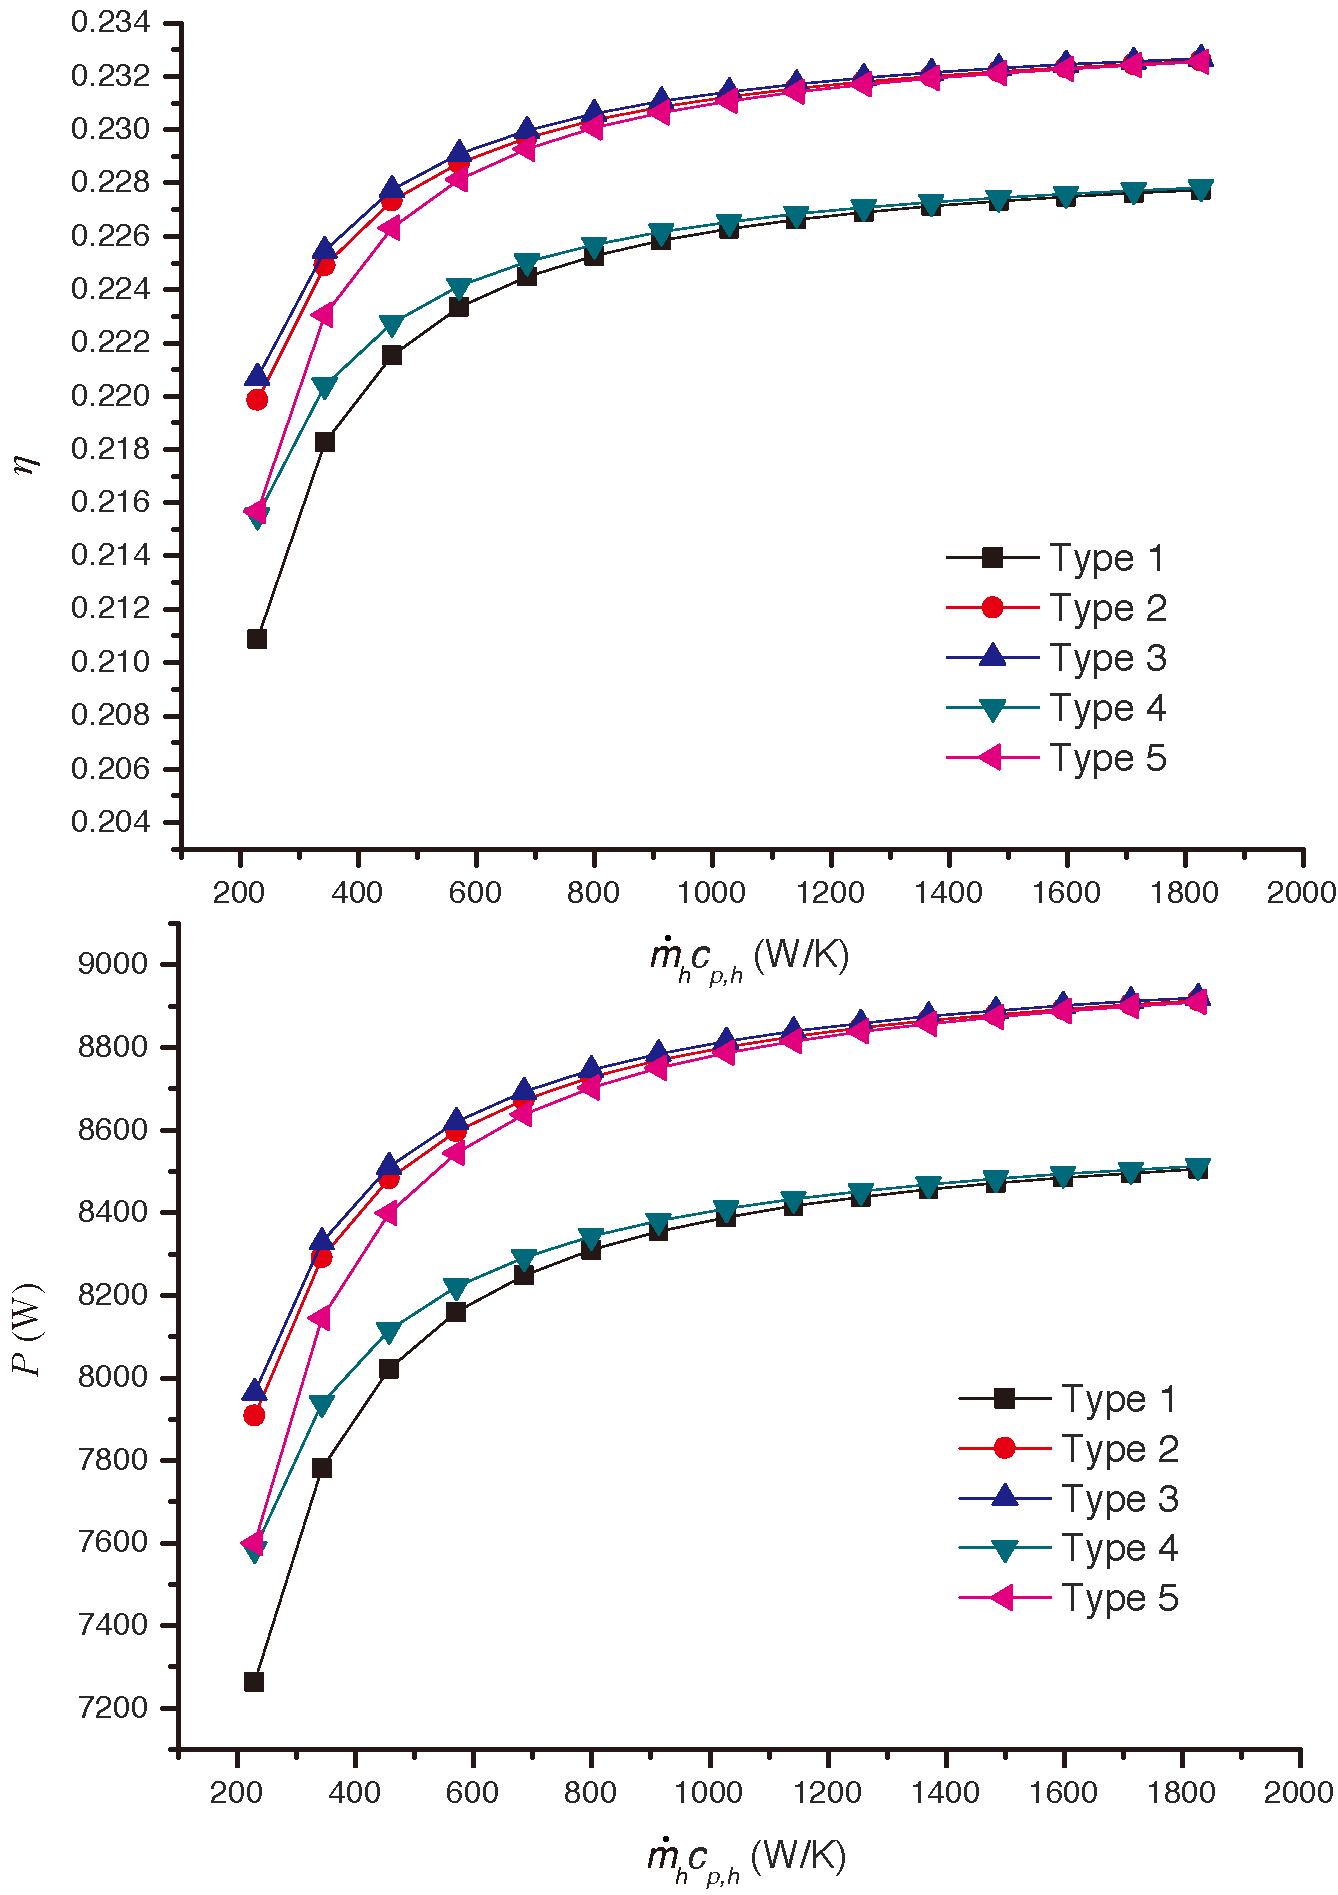
\includegraphics[width = 0.7\columnwidth]{fig/qm_hcp_h}
	\caption{Influence of $\dot{m}_hc_{p,h}$ on efficiency and power of SEA}
	\label{fig:qm_hcp_h}
\end{center}
\end{figure}

Curves of performance of SEAs and $\dot{m}_hc_{p,h}$ are shown in Figure~\ref{fig:qm_hcp_h}.
%For a connection type of SEA, $\dot{m}_hc_{p,h}$ has little effect on the performance of the SEA if it is big enough to drive the engines. This means increase the mass flow rate of heating fluid will not increase the efficiency and power of SEA significantly. 
For a large $\dot{m}_hc_{p,h}$ ($>$ 800 W/K), Type 2 , Type 3 and Type 5 have similar performance, which can be interpreted as the cooling fluid has the same properties for the two types of SEAs, and for a large $\dot{m}_hc_{p,h}$, the heating fluid has similar effect after diverged. Similar performance of Type 1 and Type 4 can be also interpreted for the same reason.

\noindent \begin{figure}[htbp]
\begin{center}
	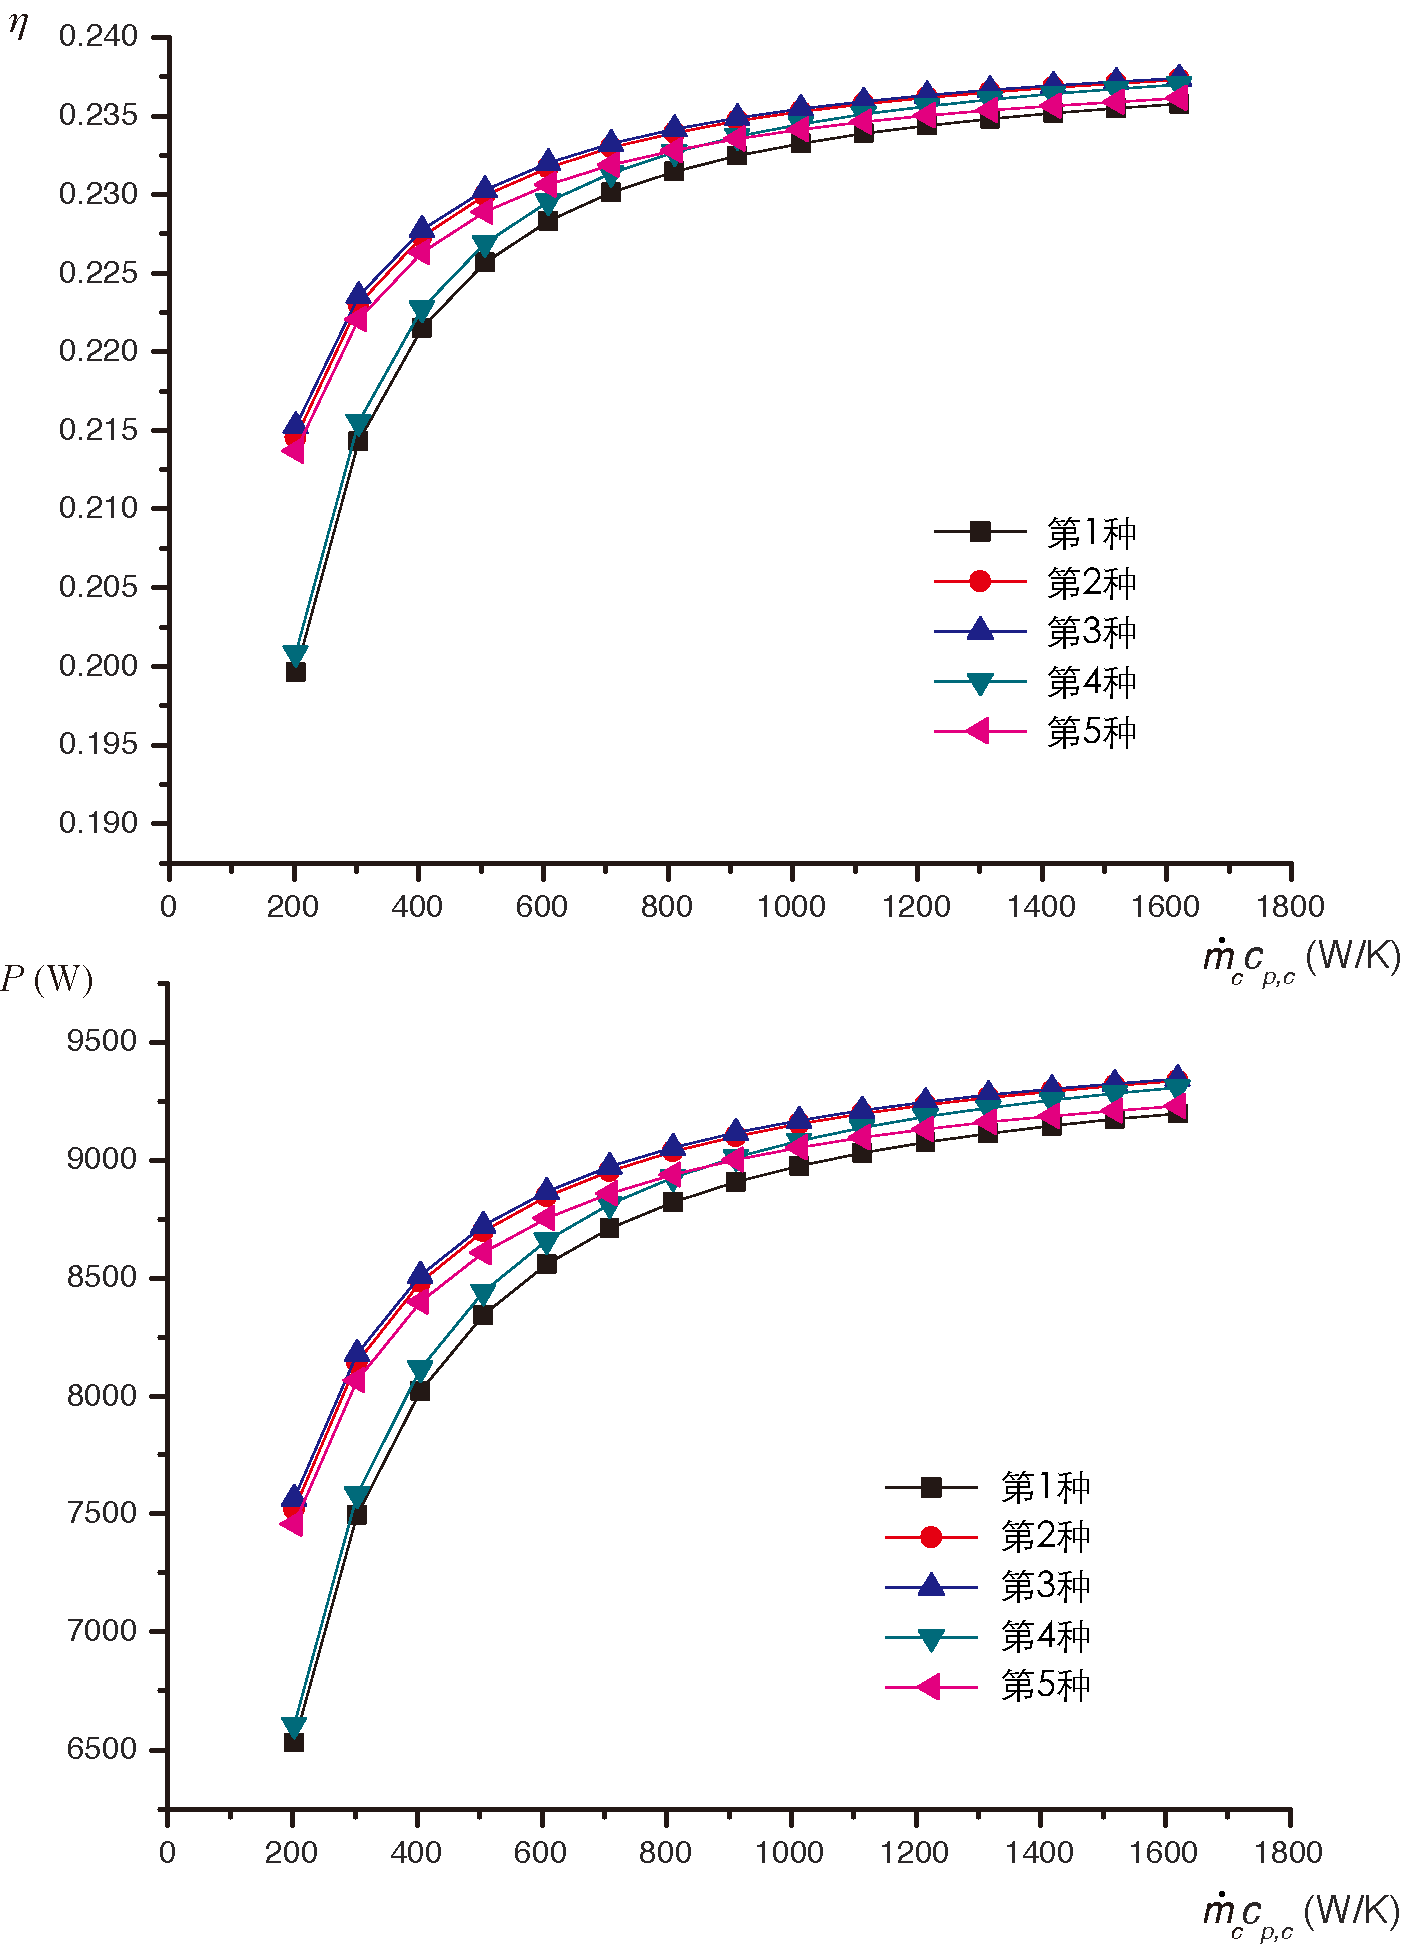
\includegraphics[width = 0.7\columnwidth]{fig/qm_ccp_c}
	\caption{Influence of $\dot{m}_cc_{p,c}$ on efficiency and power of SEA}
	\label{fig:qm_ccp_c}
\end{center}
\end{figure}

Curves of performance of SEAs and $\dot{m}_cc_{p,c}$ are shown in Figure~\ref{fig:qm_ccp_c}. For a connection type of SEA, the performance improves with the increase of $\dot{m}_cc_{p,c}$. For a large $\dot{m}_cc_{p,c}$ ($>$ 800 W/K), Type 2 and Type 3 have similar performance, which means the flow order doesn't affect the performance of SEA with a large $\dot{m}_cc_{p,c}$. There exists an intersection point (at 830 W/K) of curves of Type 4 and Type 5. For a larger $\dot{m}_cc_{p,c}$, Type 4 has a better performance, and vice versa. This can be interpreted that larger $\dot{m}_cc_{p,c}$ weaken the drawback of larger temperature rise of parallel flow, while for the heating fluid, temperature drop of serial flow is smaller than parallel flow.

\subsection{Effects of $n_{se}$}

By varying the number of engines in SEA, the performance levels changed accordingly. $n_{se}$ may affect both the flow rates and temperatures of fluids of each engine. Figure~\ref{fig:n_se} shows curves of performance of SEAs with different $n_{se}$. As it is shown, with an increase of $n_{se}$ leads to a reduction of $\eta$ for all SEAs due to smaller heating and cooling average temperature difference for more engines. For some types of SEA, when $n_{se}$ is larger than a critical value, some of the engines in the SEA will not work and the curves will dive. E.g. for SEA of Type 1, when $n_{se}$ is larger than 9, all the engines stop working, turning points at 9 can be found on the $\eta-n_{se}$, $P-n_{se}$ curves in Figure~\ref{fig:n_se}.

\noindent \begin{figure}[htbp]
\begin{center}
	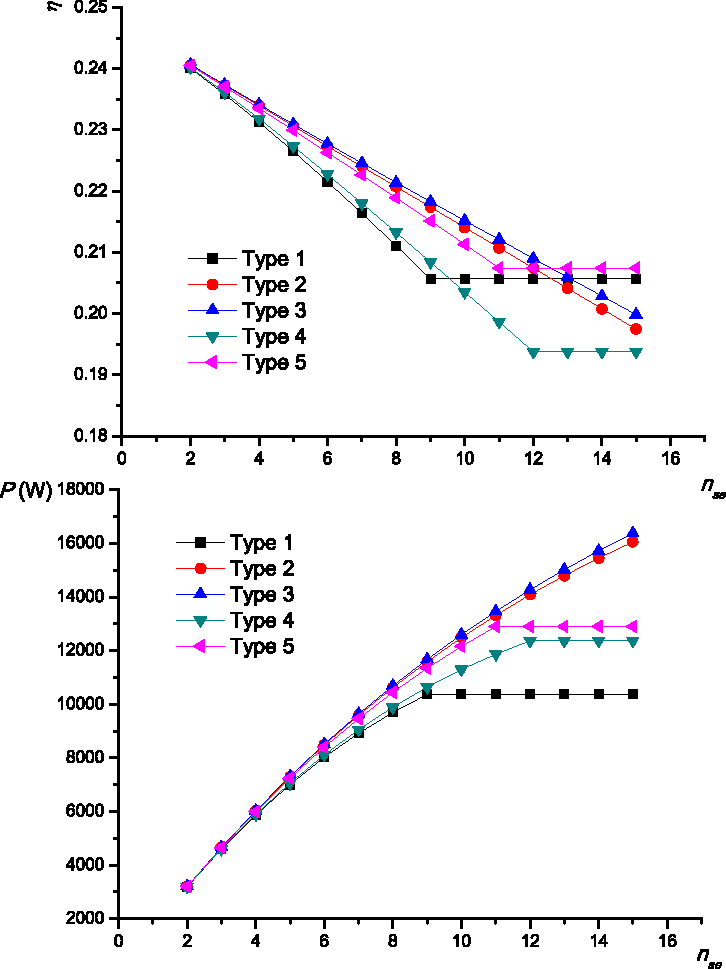
\includegraphics[width = 0.7\columnwidth]{fig/n_se}
	\caption{Influence of $n_{se}$ on efficiency and power of SEA}
	\label{fig:n_se}
\end{center}
\end{figure}

For Type 1, when $n_{se} \geqslant 10$, all engines stop working for given heating and cooling fluids due to small $\dot{m}c_p$. For Type 2 and Type 3, every engine in the SEAs works, by increasing $n_{se}$, $\eta$ reduces due to smaller temperature difference of the fluids, and $P$ increases due to more operating engines. For Type 4, by checking results, it can be found that when $n_{se} = 13$,  the last engine doesn't work; when $n_{se} = 14$, only the first 10 engines will work; when $n_{se} = 15$, the working engine number drops to 9. For Type 5, by checking results, it can be found that when $n_{se} = 12$, the last 2 engines stop working; when $n_{se} = 13$, only the first 8 engines will work; when $n_{se} = 14$, the working engine number drops to 6; when $n_{se} = 15$, the working engine number drops to 4.

For a certain connection type, increase $n_{se}$ will reduce the efficiency of SEA. For some connection types, increase $n_{se}$ will reduce the output power $P$ due to inoperative engines and smaller output power engines. It is important to choose the number of engines for some connection types of SEA. 

\section{Conclusion}

A new layout scheme of the solar dish system by using SEA were proposed in this thesis. Connection type of the engines may change the flow rates and temperatures of the fluids, as a result the performance of the SEA will be different depending on the connection schemes. In order to compare performance of SEAs with different arrangements, five basic connection types of SEA were summed up according to flow type and flow order. 

%Analytical Stirling engine model was created to develop the SEA models for the investigation of influence of connection types. Imperfect regeneration and cycle irreversibility of Stirling engine cycle and heat exchange process between fluids and engine were considered in the model. Algorithm to numerically solve different connection types of SEA was developed. The model was evaluated by considering the prototype GPU-3 Stirling engine as a case study. Result shows that the proposed model predicted the performance with higher accuracy than Simple model~\cite{Urieli1984} and Simple II model~\cite{Strauss2010}. 

Models of SEAs were developed to calculated the performance under different parameters to find out the impacts of $T_{i,h}$, $\dot{m}_hc_{p,h}$, $\dot{m}_cc_{p,c}$ and $n_{se}$ on different connection types. It was found that, as expected, decrease $T_{i,h}$ and $\dot{m}c_{p}$ will weaken the performance of SEA of all connection types. However, for some connection types, there exists a critical temperature below which some engines stop working. This needs to be considered for SEA connection type selection, especially when $T_{i,h}$ is low. For given heating and cooling fluids, Type 2 has the best performance and adaptability. Type 2 and Type 3 have similar performance under different parameters ($T_{i,h}$, $T_{i,c}$ and $\dot{m}c_p$), which means the flow order has little influence on the performance of an SEA. SEA of serial flows (Type 3) has the best performance and adaptability under different parameters. Given heating and cooling fluids, using serial flow is the best choice for the connection type of an SEA. %This means the new arrangement of dish-Stirling system in Figure~\ref{fig:Dish_SEA} may have better performance than the traditional arrangement, which can be considered as a particular case of Type 1.

%It is important to note that, in the future researches, the experiments of influence of connection type on SEA's performance can be carried out to verify the conclusions in this thesis.